\section{Benutzerschnittstelle}

\subsection{Einführung}
Die Benutzeroberfläche muss so aufgebaut sein, dass auch unerfahrene Benutzer das System problemlos verwenden können.
Um die Benutzerführung zu optimieren werden insbesondere sog. "Wizards" verwendet, in welchen der Benutzer dann durch die verschiedenen Schritte eines gegebenen Ablaufs geführt wird. Darüber hinaus wird an vielen Stellen das Drag-and-Drop-Konzept verwendet, um so die Oberfläche intuitiver zu gestalten und die Dauer der einzelnen Interaktionen zu verkürzen.

\subsection{Login}
\begin{figure}[!htb]
	\caption{Loginseite des Systems mit Anmeldung über den Shibboleth Identity Provider des KITs}
	\label{fig:gui-login-1}
	\centering
	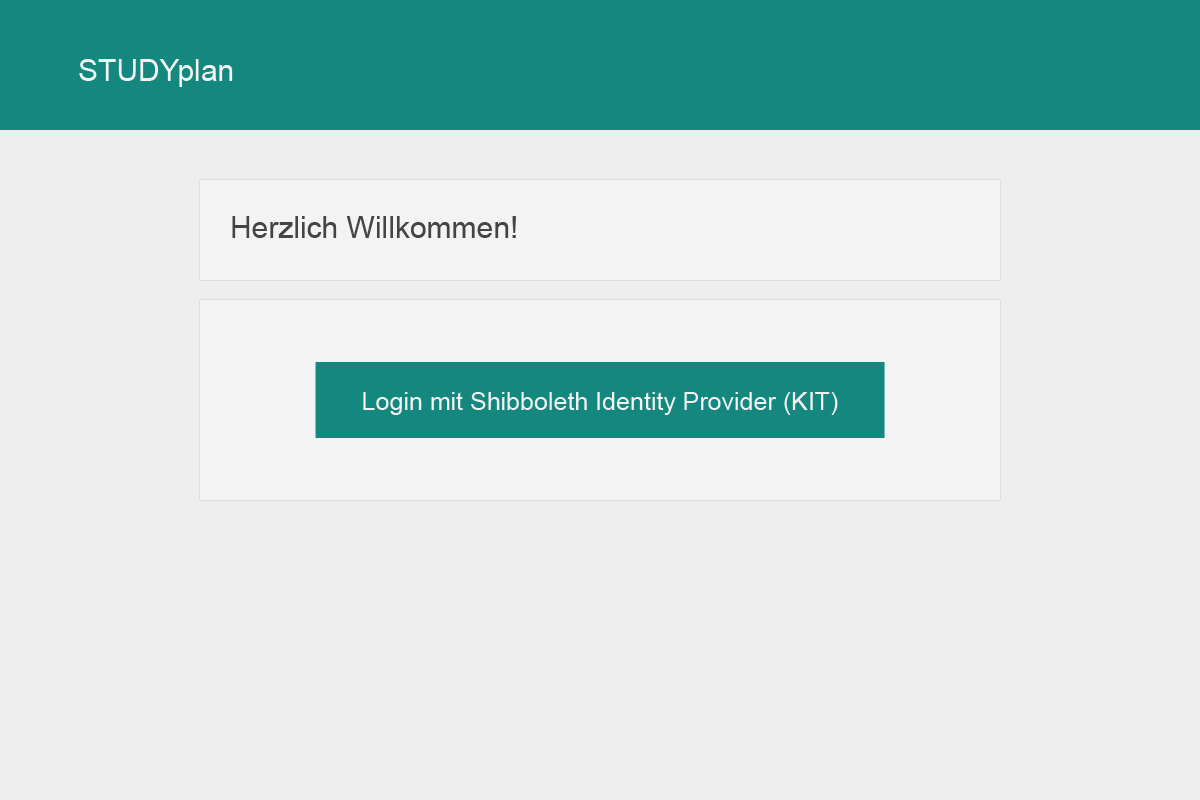
\includegraphics[width=0.7\textwidth]{../GUI/ergebnisse/login-1.png}
\end{figure}
Das ist jetzt mal hier so ein Test. Bitte einfach ignorieren.
Abbildung \ref{fig:gui-login-1} zeigt die Login-Seite.
\subsection{Registrierungs-Wizard}
Das ist ein Test
\begin{figure}[!htb]
	\caption{}
	\label{fig:gui-registrierung-1}
	\centering
	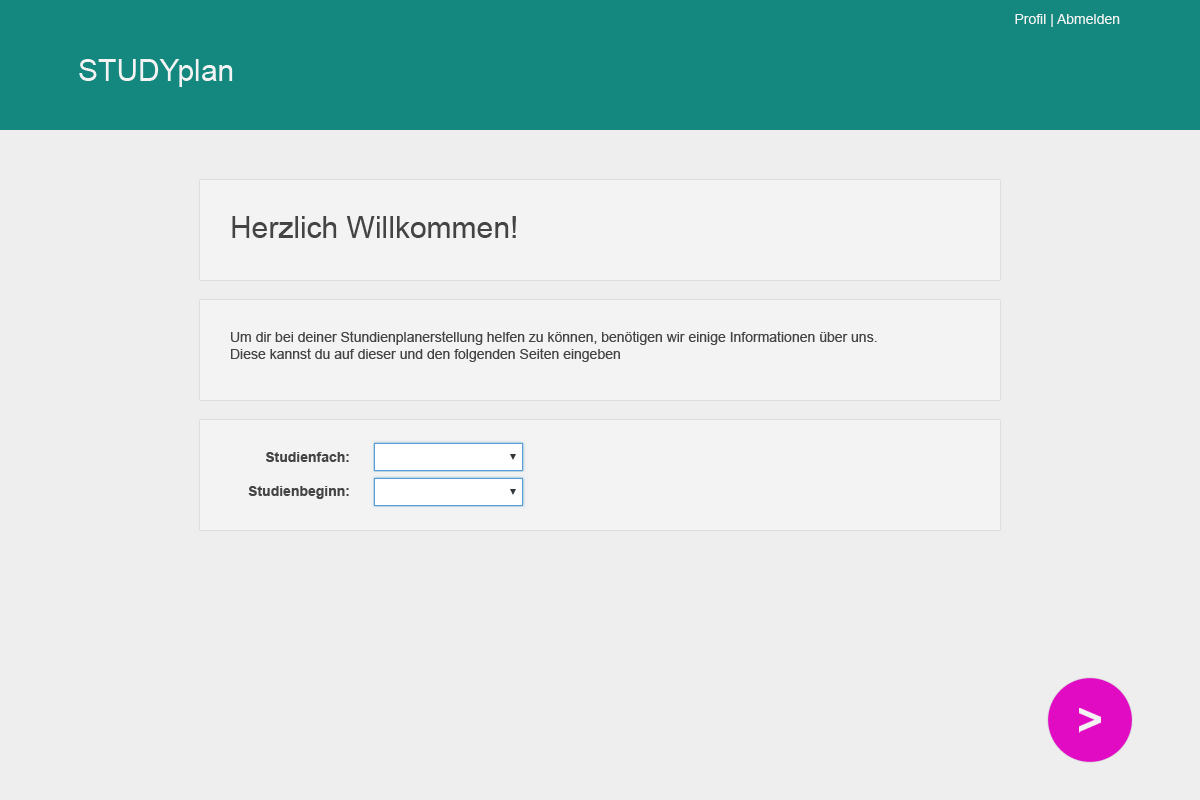
\includegraphics[width=0.7\textwidth]{../GUI/ergebnisse/registrierung-1.png}
\end{figure}

\begin{figure}[!htb]
	\caption{}
	\label{fig:gui-registrierung-2}
	\centering
	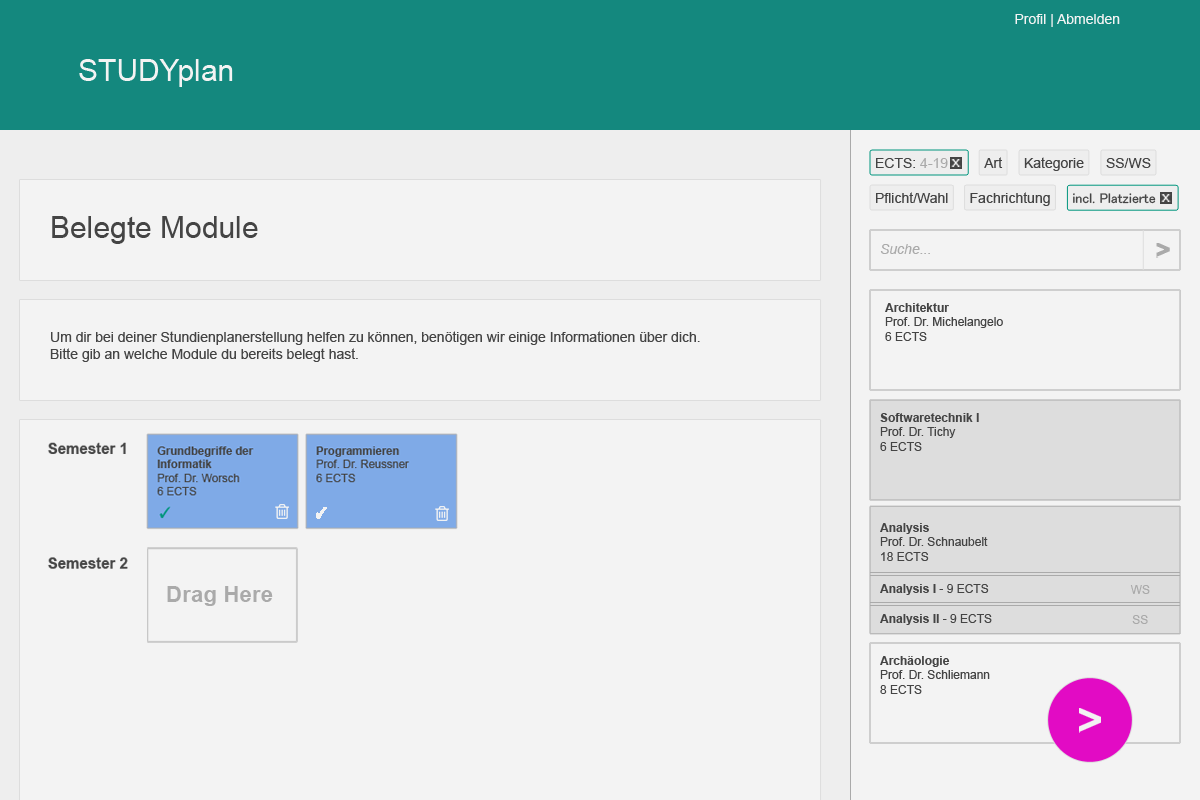
\includegraphics[width=0.7\textwidth]{../GUI/ergebnisse/registrierung-2.png}
\end{figure}


\subsection{Hauptseite}
Das ist die Hauptseite.
\begin{figure}[!htb]
	\caption{}
	\label{fig:gui-hauptseite-1}
	\centering
	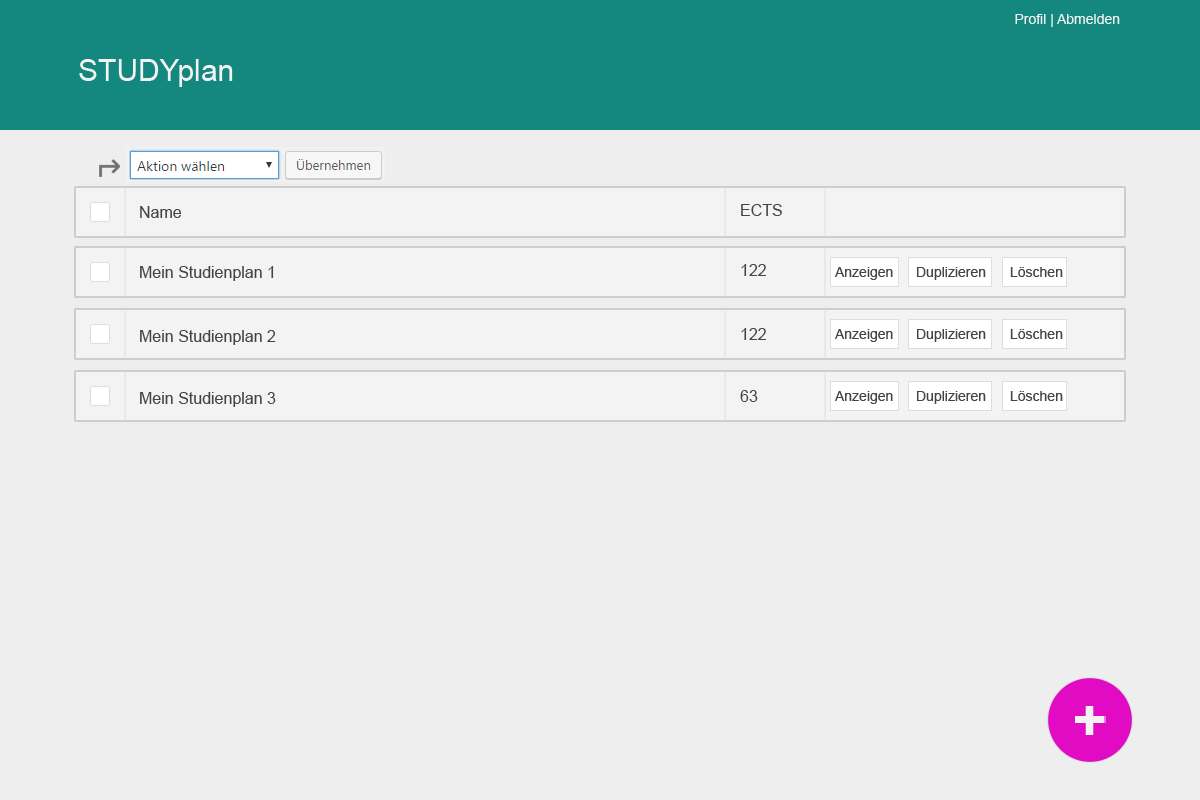
\includegraphics[width=0.7\textwidth]{../GUI/ergebnisse/hauptseite-1.png}
\end{figure}

\subsection{Manuelle Studienplan-Bearbeitung}
Manuelle Bearbeitung.
\begin{figure}[!htb]
	\caption{}
	\label{fig:gui-bearbeitung-1}
	\centering
	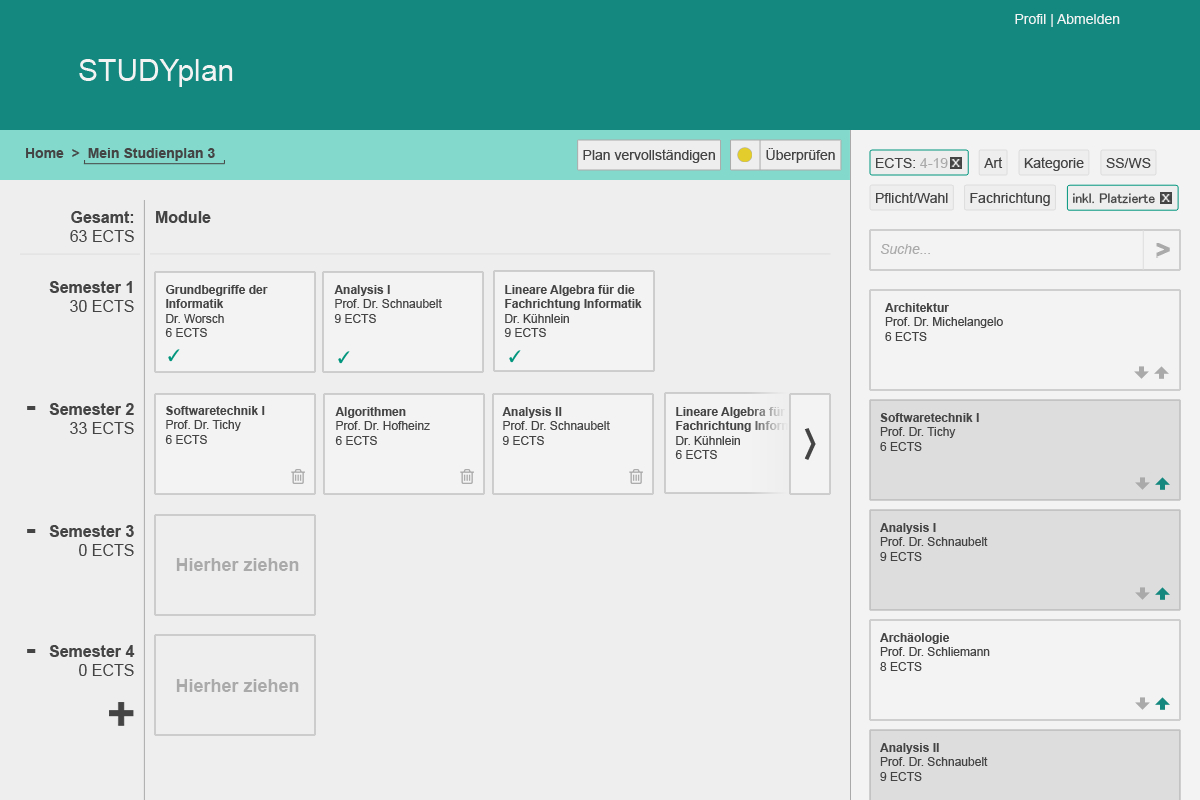
\includegraphics[width=0.7\textwidth]{../GUI/ergebnisse/bearbeitung-1.png}
\end{figure}

\subsubsection{Module filtern}
Module sind filterbar.
\begin{figure}[!htb]
	\caption{}
	\label{fig:gui-module-filtern-1}
	\centering
	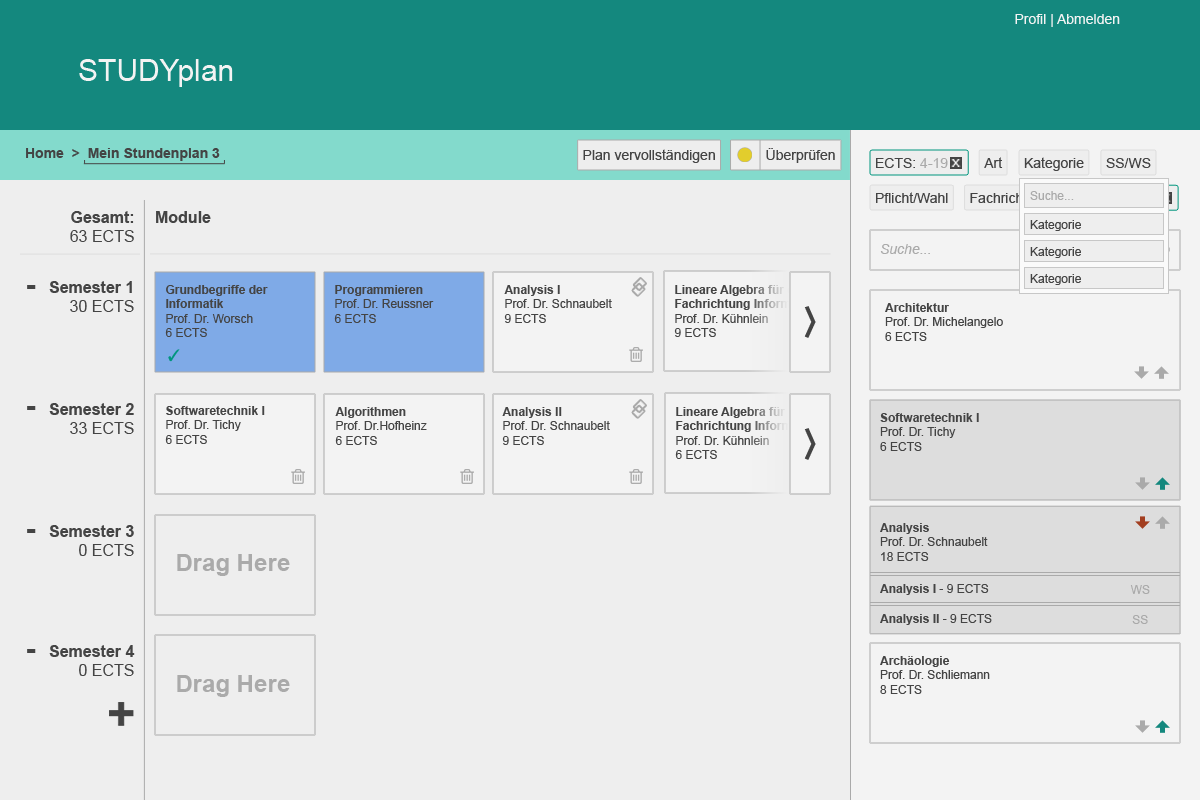
\includegraphics[width=0.7\textwidth]{../GUI/ergebnisse/module-filtern-1.png}
\end{figure}
\begin{figure}[!htb]
	\caption{}
	\label{fig:gui-module-filtern-2}
	\centering
	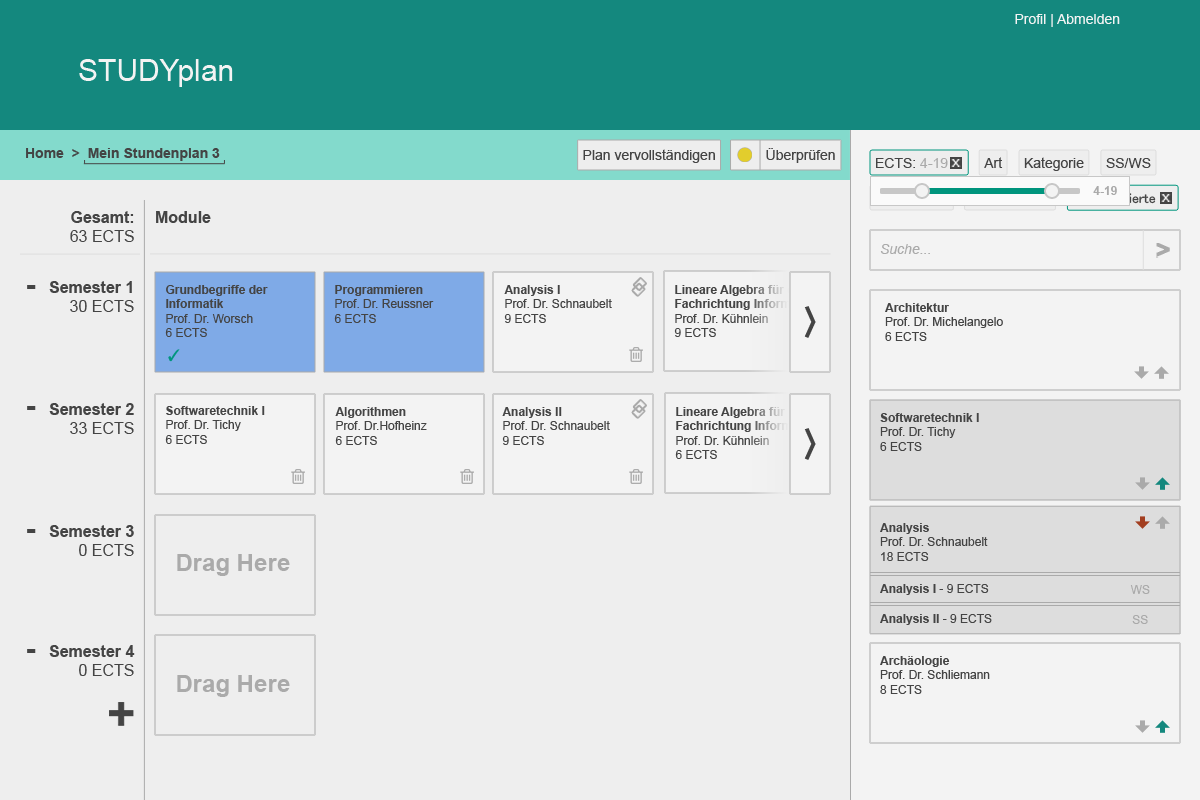
\includegraphics[width=0.7\textwidth]{../GUI/ergebnisse/module-filtern-2.png}
\end{figure}

\subsubsection{Modul-Informationen anzeigen}
Modulinformationen lassen sich auch anzeigen
\begin{figure}[!htb]
	\caption{}
	\label{fig:gui-modul-info-1}
	\centering
	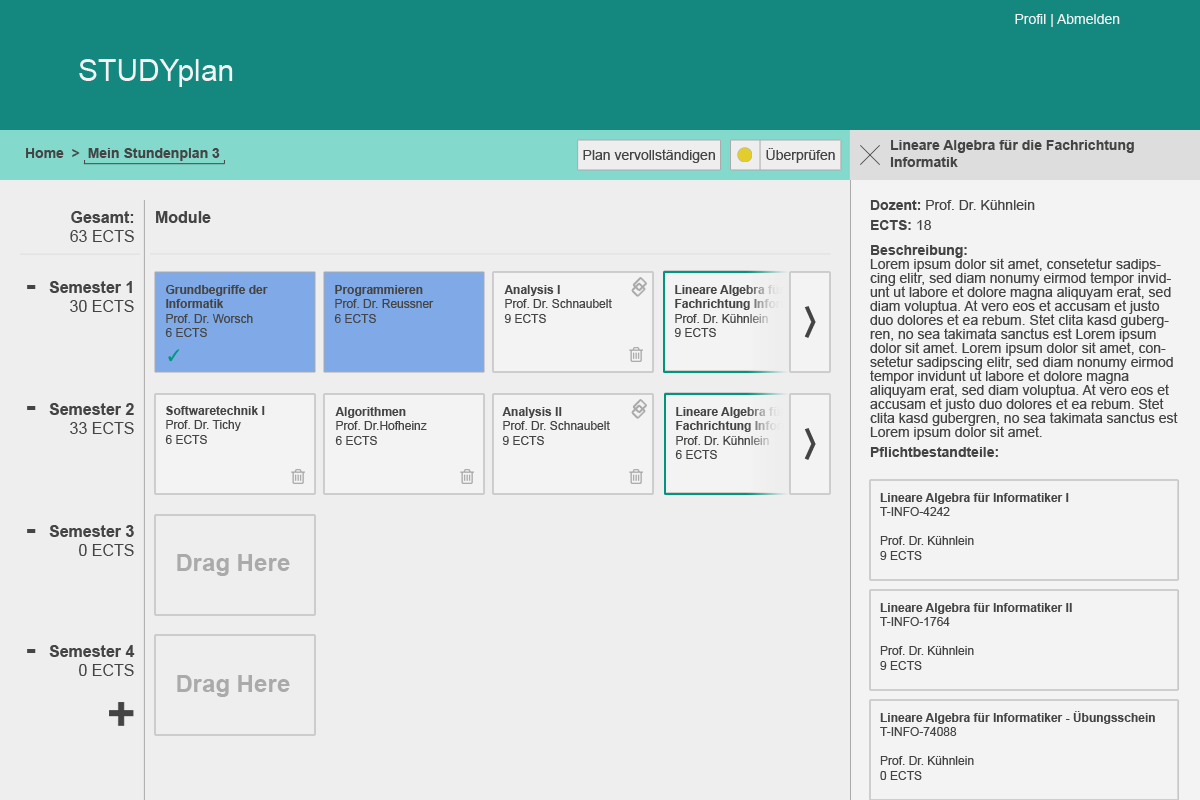
\includegraphics[width=0.7\textwidth]{../GUI/ergebnisse/modul-info-1.png}
\end{figure}


\subsection{Generierungs-Wizard}
Hier kann man Stundenpläne generieren.
\begin{figure}[!htb]
	\caption{}
	\label{fig:gui-generierung-1}
	\centering
	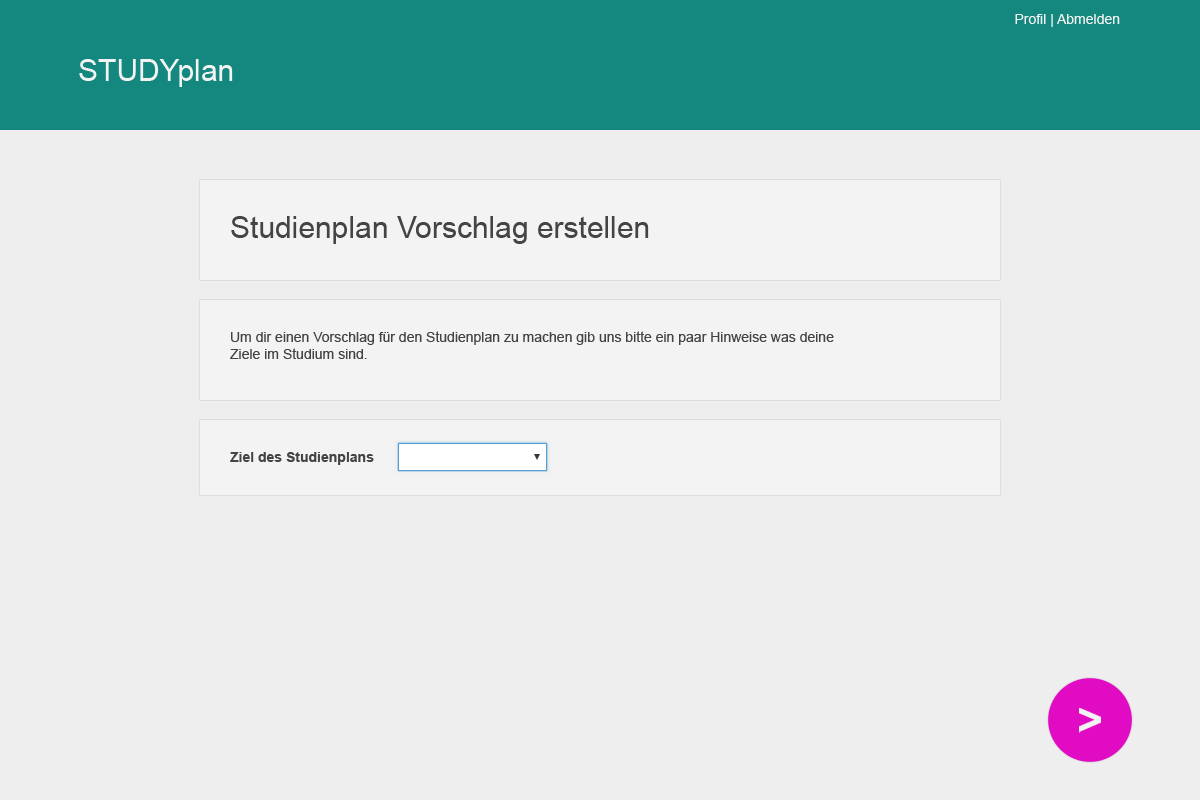
\includegraphics[width=0.7\textwidth]{../GUI/ergebnisse/generierung-1.png}
\end{figure}

\begin{figure}[!htb]
	\caption{}
	\label{fig:gui-generierung-2}
	\centering
	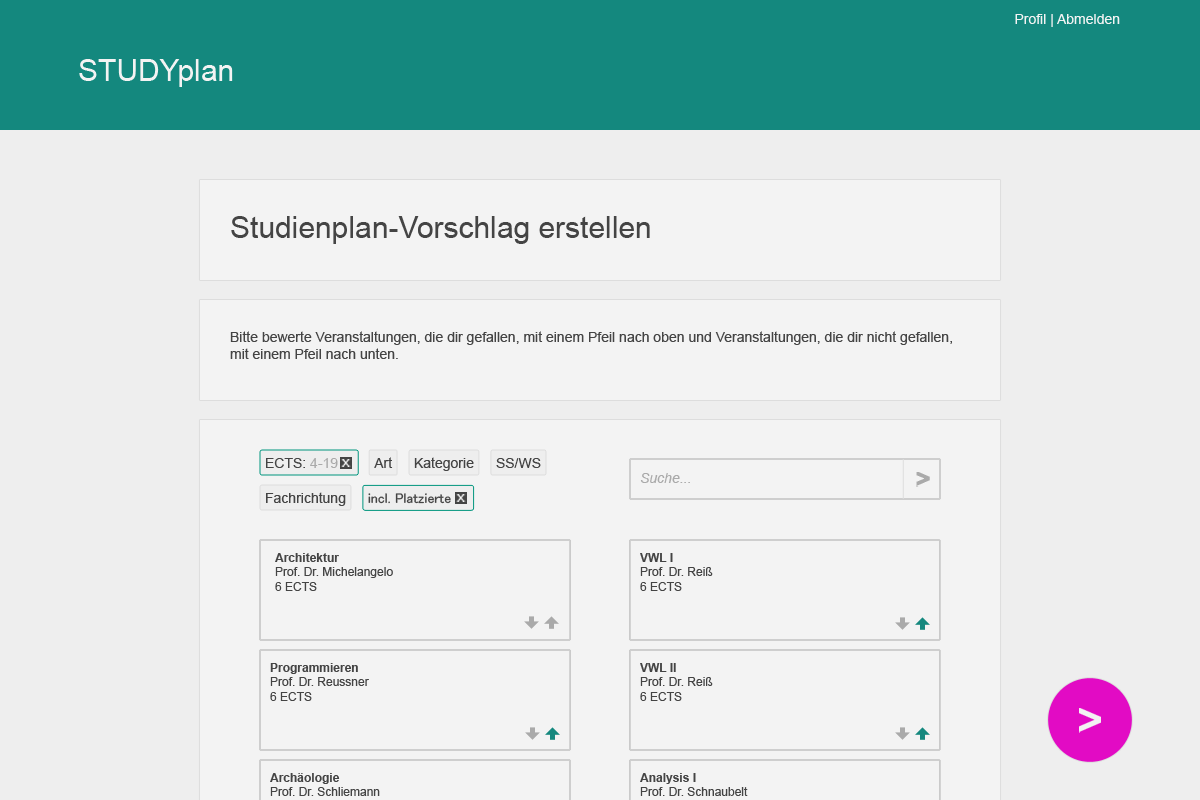
\includegraphics[width=0.7\textwidth]{../GUI/ergebnisse/generierung-2.png}
\end{figure}

\begin{figure}[!htb]
	\caption{}
	\label{fig:gui-generierung-3}
	\centering
	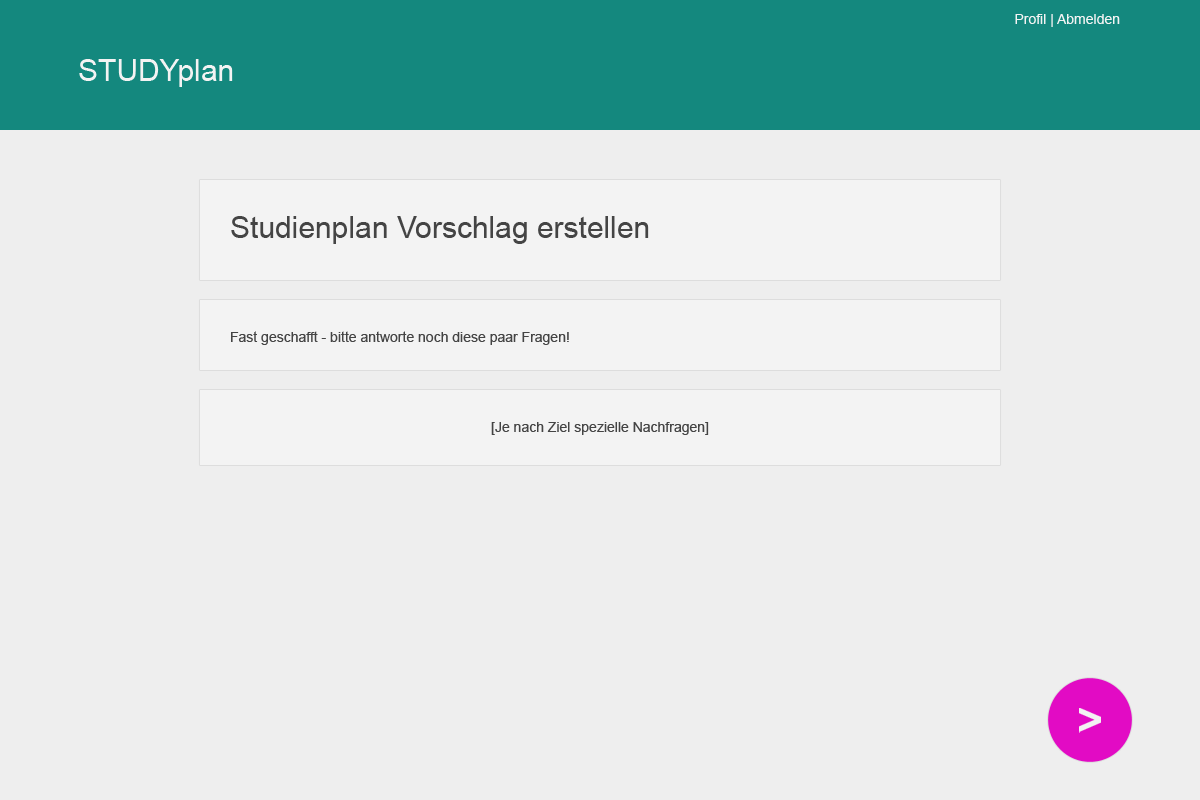
\includegraphics[width=0.7\textwidth]{../GUI/ergebnisse/generierung-3.png}
\end{figure}

\begin{figure}[!htb]
	\caption{}
	\label{fig:gui-generierung-4}
	\centering
	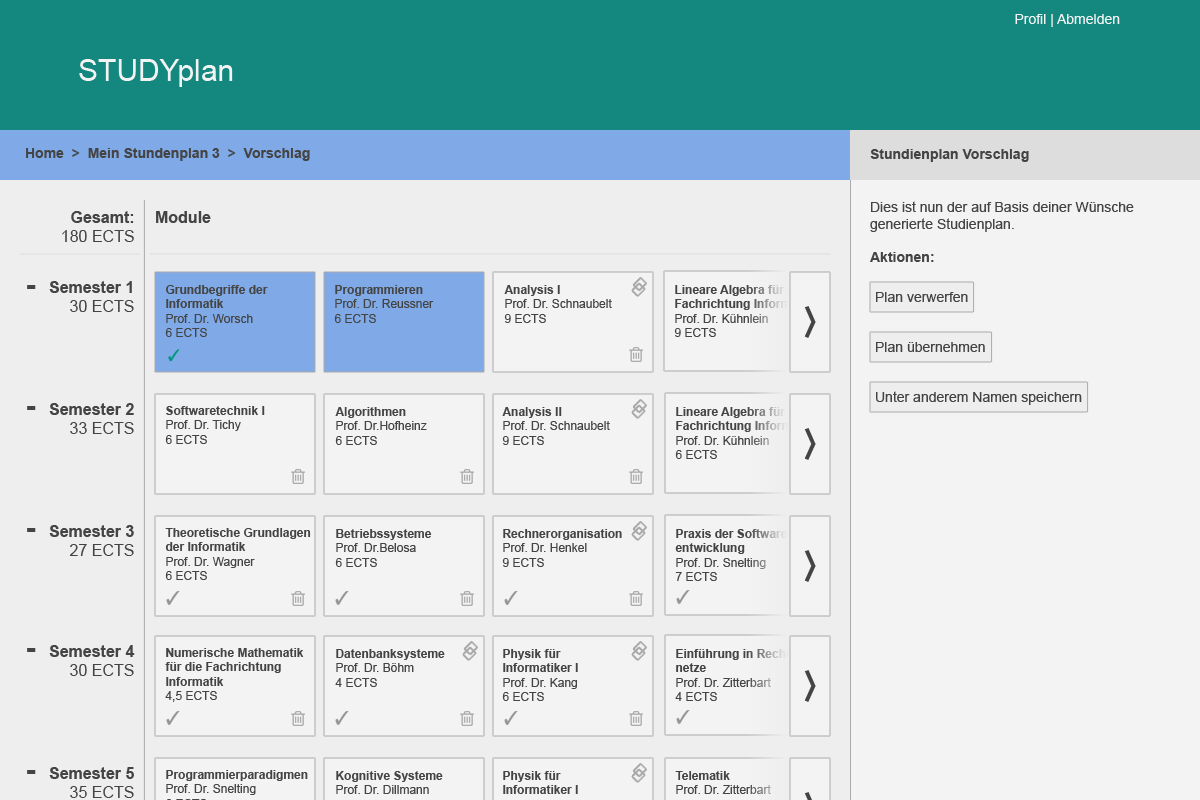
\includegraphics[width=0.7\textwidth]{../GUI/ergebnisse/generierung-4.png}
\end{figure}

\subsection{Verifizierung}
Verifizierung ist auch möglich mittels dieser Darstellung.
\begin{figure}[!htb]
	\caption{}
	\label{fig:gui-verifizierung-1}
	\centering
	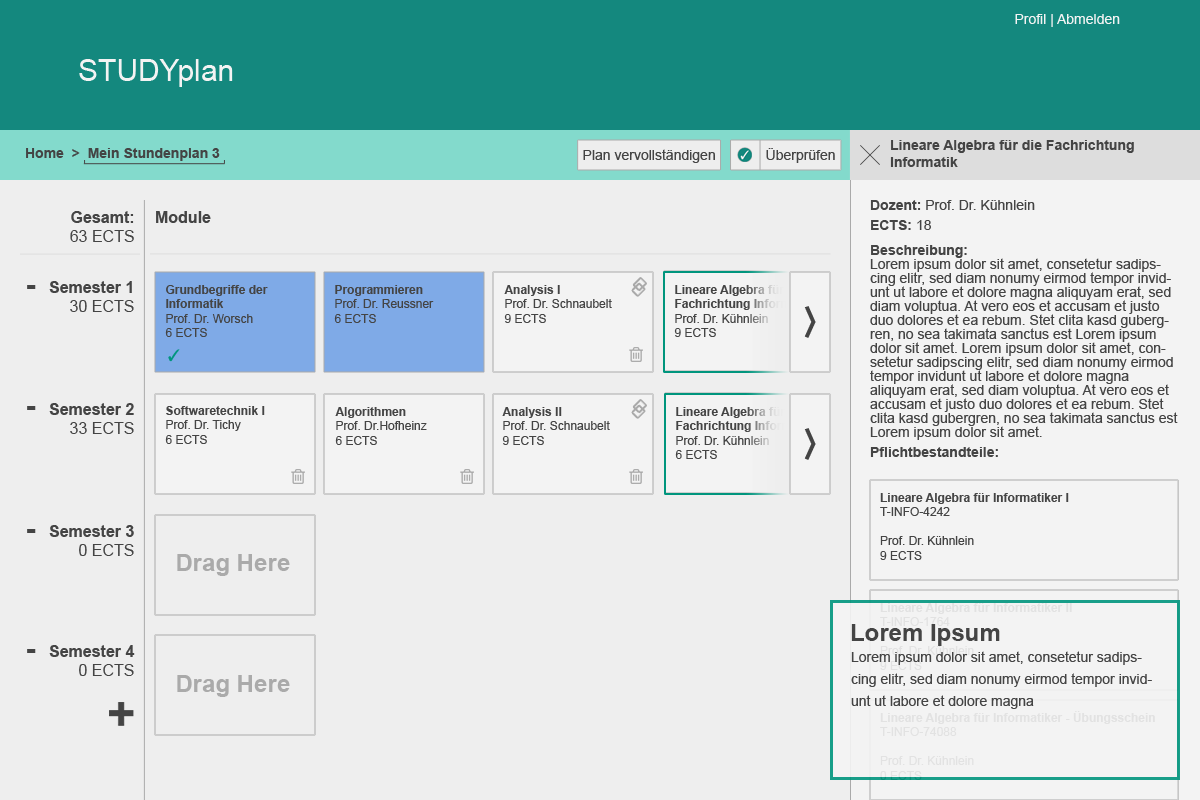
\includegraphics[width=0.7\textwidth]{../GUI/ergebnisse/verifizierung-1.png}
\end{figure}
\begin{figure}[!htb]
	\caption{}
	\label{fig:gui-verifizierung-2}
	\centering
	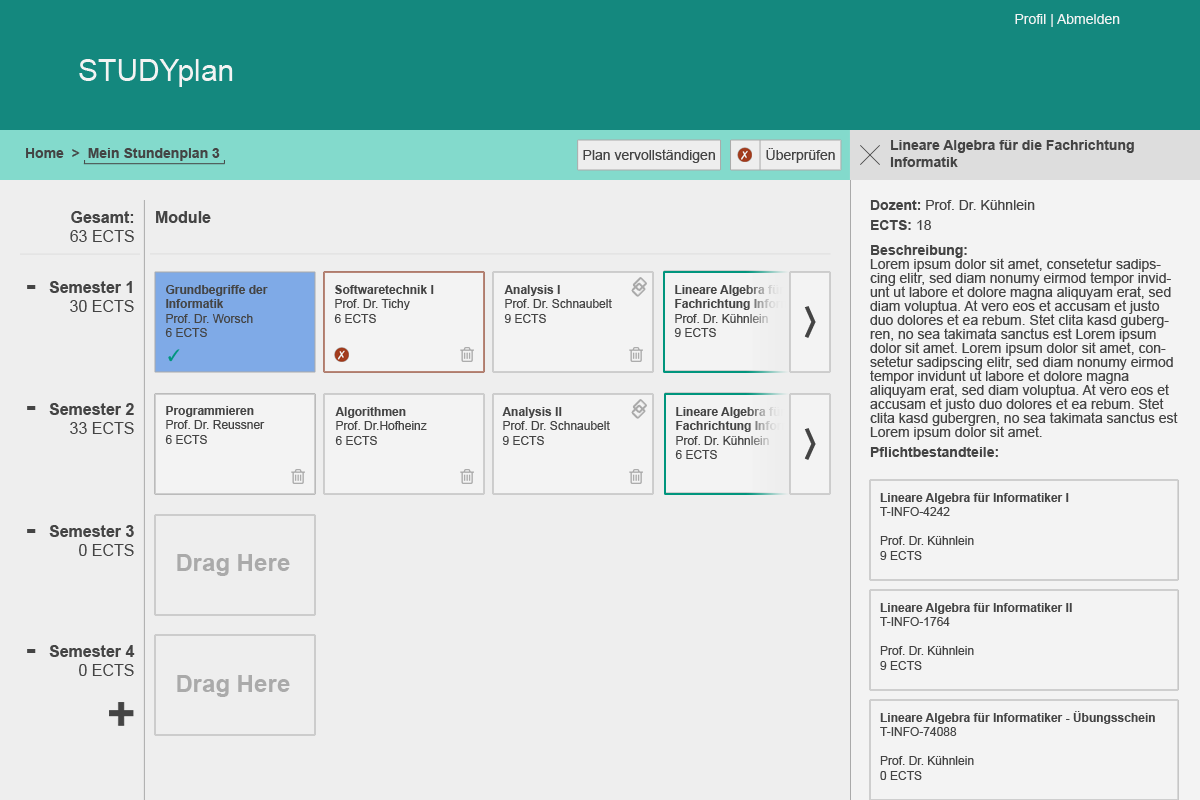
\includegraphics[width=0.7\textwidth]{../GUI/ergebnisse/verifizierung-2.png}
\end{figure}

\subsection{Profil}
So sieht das Profil aus.
\begin{figure}[!htb]
	\caption{}
	\label{fig:gui-profil-1}
	\centering
	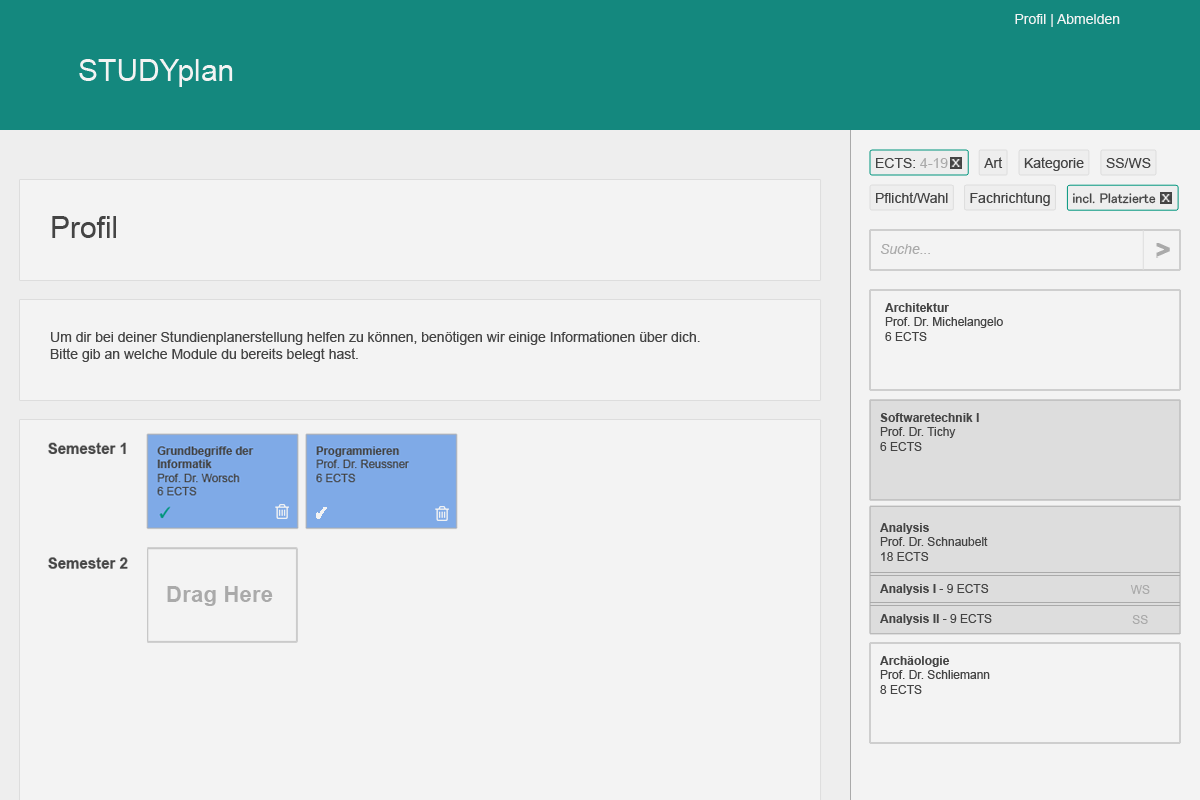
\includegraphics[width=0.7\textwidth]{../GUI/ergebnisse/profil-1.png}
\end{figure}